\documentclass[12pt]{article}\usepackage[]{graphicx}\usepackage[]{color}
% maxwidth is the original width if it is less than linewidth
% otherwise use linewidth (to make sure the graphics do not exceed the margin)
\makeatletter
\def\maxwidth{ %
  \ifdim\Gin@nat@width>\linewidth
    \linewidth
  \else
    \Gin@nat@width
  \fi
}
\makeatother

\definecolor{fgcolor}{rgb}{0.345, 0.345, 0.345}
\newcommand{\hlnum}[1]{\textcolor[rgb]{0.686,0.059,0.569}{#1}}%
\newcommand{\hlstr}[1]{\textcolor[rgb]{0.192,0.494,0.8}{#1}}%
\newcommand{\hlcom}[1]{\textcolor[rgb]{0.678,0.584,0.686}{\textit{#1}}}%
\newcommand{\hlopt}[1]{\textcolor[rgb]{0,0,0}{#1}}%
\newcommand{\hlstd}[1]{\textcolor[rgb]{0.345,0.345,0.345}{#1}}%
\newcommand{\hlkwa}[1]{\textcolor[rgb]{0.161,0.373,0.58}{\textbf{#1}}}%
\newcommand{\hlkwb}[1]{\textcolor[rgb]{0.69,0.353,0.396}{#1}}%
\newcommand{\hlkwc}[1]{\textcolor[rgb]{0.333,0.667,0.333}{#1}}%
\newcommand{\hlkwd}[1]{\textcolor[rgb]{0.737,0.353,0.396}{\textbf{#1}}}%
\let\hlipl\hlkwb

\usepackage{framed}
\makeatletter
\newenvironment{kframe}{%
 \def\at@end@of@kframe{}%
 \ifinner\ifhmode%
  \def\at@end@of@kframe{\end{minipage}}%
  \begin{minipage}{\columnwidth}%
 \fi\fi%
 \def\FrameCommand##1{\hskip\@totalleftmargin \hskip-\fboxsep
 \colorbox{shadecolor}{##1}\hskip-\fboxsep
     % There is no \\@totalrightmargin, so:
     \hskip-\linewidth \hskip-\@totalleftmargin \hskip\columnwidth}%
 \MakeFramed {\advance\hsize-\width
   \@totalleftmargin\z@ \linewidth\hsize
   \@setminipage}}%
 {\par\unskip\endMakeFramed%
 \at@end@of@kframe}
\makeatother

\definecolor{shadecolor}{rgb}{.97, .97, .97}
\definecolor{messagecolor}{rgb}{0, 0, 0}
\definecolor{warningcolor}{rgb}{1, 0, 1}
\definecolor{errorcolor}{rgb}{1, 0, 0}
\newenvironment{knitrout}{}{} % an empty environment to be redefined in TeX

\usepackage{alltt}
%Required: You must have these
\usepackage{graphicx}
\usepackage{tabularx}
\usepackage{natbib}
\usepackage{pdflscape}
\usepackage{array}
\usepackage{authblk}
\usepackage{gensymb}
\usepackage{amsmath}
%\usepackage[backend=bibtex]{biblatex}
\usepackage[small]{caption}

\setkeys{Gin}{width=0.8\textwidth}
\setlength{\captionmargin}{30pt}
\setlength{\abovecaptionskip}{10pt}
\setlength{\belowcaptionskip}{10pt}

 \topmargin -1.5cm 
 \oddsidemargin -0.04cm 
 \evensidemargin -0.04cm 
 \textwidth 16.59cm
 \textheight 21.94cm 
 \parskip 7.2pt 
\renewcommand{\baselinestretch}{1.6} 	
\parindent 0pt
\usepackage{setspace}
\usepackage{lineno}
\title{Plum update}
\author{Buonaiuto, Collins, Wolkovich}
\IfFileExists{upquote.sty}{\usepackage{upquote}}{}
\begin{document}
\maketitle
\subsection{Basic model}
\begin{itemize}
\item subset data to include only observations of flowers (BBCH 60-67) [could drop to 65]
\item model: $BBCH.v \sim doy.observation.centered + (1|species)$.\\
In this situation we are ``controling for" doy. Performed a LOO comparision vs. Intercept only, and pooling on slopes and intercepts. I also ran a no-pooling model for species only to understand how the partial pooling is impacting results.
\item Ran several different kinds of models. 
\begin{itemize}
\item Gaussian with BBCH as is (7,9,11,15,17 etc)
\item Gaussian with scaled BBCH (0,1,2,3,4 etc)
\item Poission with scaled BBCH
\item Oridnal (cumuliative distrubution with logit link function)
\end{itemize}
\end{itemize}
    
\subsection{Trait correlation and hypotheses}
\begin{itemize}
\item pdsi (drought tolerance hypothesis)
\item petal length (insect visibility hypothesis)
\item fruit diameter (early flowering hypothesis)
\item min T (drought tolerance to cold tolderance hypothesis)
\item soil type (drought tolerance or resource allocation)
\item phylogeny (emailed Joey Shaw on 14 DEC 2020 for newick file...no response)
\end{itemize}

\subsection{Some plots}
\begin{figure}[h!]
        \centering
         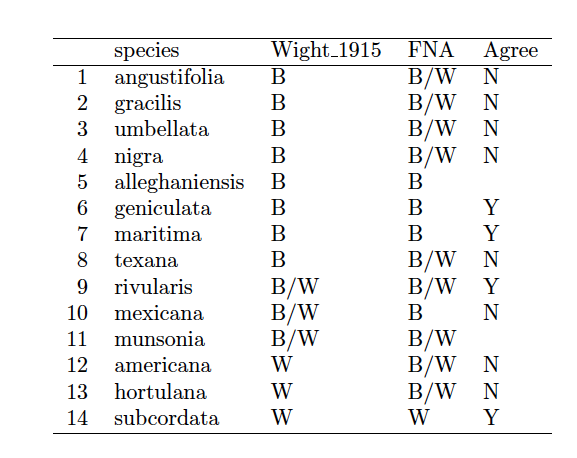
\includegraphics[width=\textwidth]{..//Plots/comparison_table.png}
                 \caption{The two main sources that describe FLS in American plums do it pretty differenty}
    \end{figure}  

\begin{figure}[h!]
        \centering
         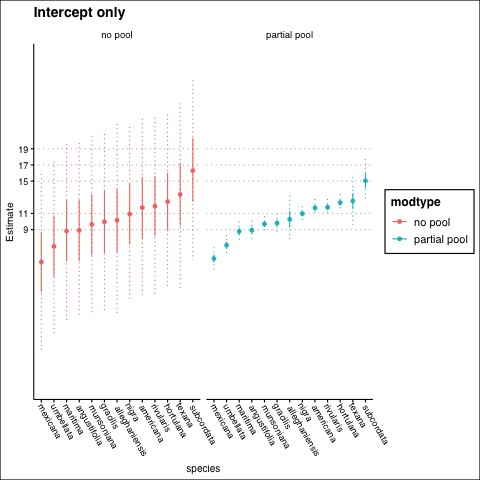
\includegraphics[width=\textwidth]{..//Plots/poolingcomps.jpeg}
                 \caption{Basic model comparing no-pooling and partial-pooling. Seems like the uncertainty intervals are the main differences}
    \end{figure}  
    
    \begin{figure}[h!]
        \centering
         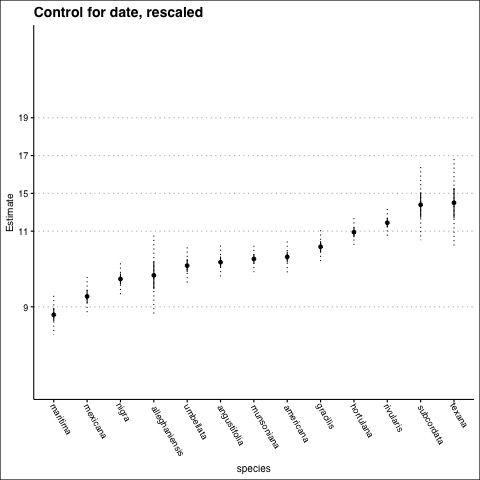
\includegraphics[width=\textwidth]{..//Plots/seeminglybestplot_rescaled.jpeg}
                 \caption{This is gaussian rescaled (BBCH 0,1,2,3 etc), but y axis transfored back to origianl BBCH. Controling for DOY.}
    \end{figure}  
    
     \begin{figure}[h!]
        \centering
         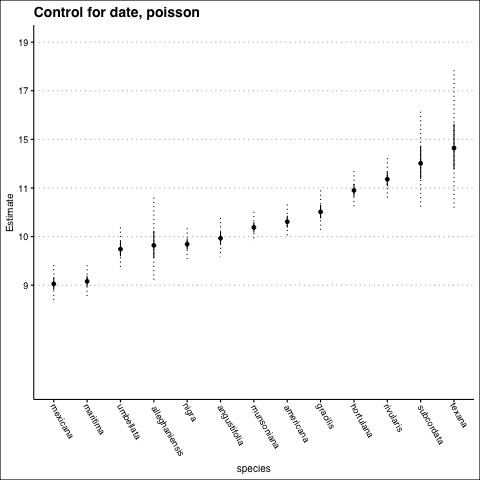
\includegraphics[width=\textwidth]{..//Plots/seeminglybestplot_poisson.jpeg}
                 \caption{Same as above but poisson}
    \end{figure}
    
       \begin{figure}[h!]
        \centering
         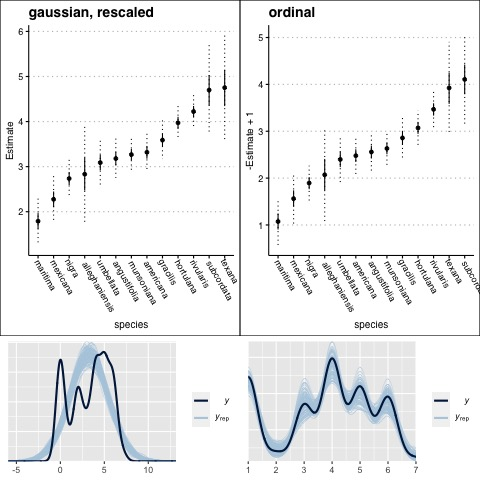
\includegraphics[width=\textwidth]{..//Plots/ordinal_reg.jpeg}
                 \caption{Ordinal vs. rescaled gaussian. (need to fix y axes)}
    \end{figure}

\subsection*{Teaser}
   \begin{figure}[h!]
        \centering
         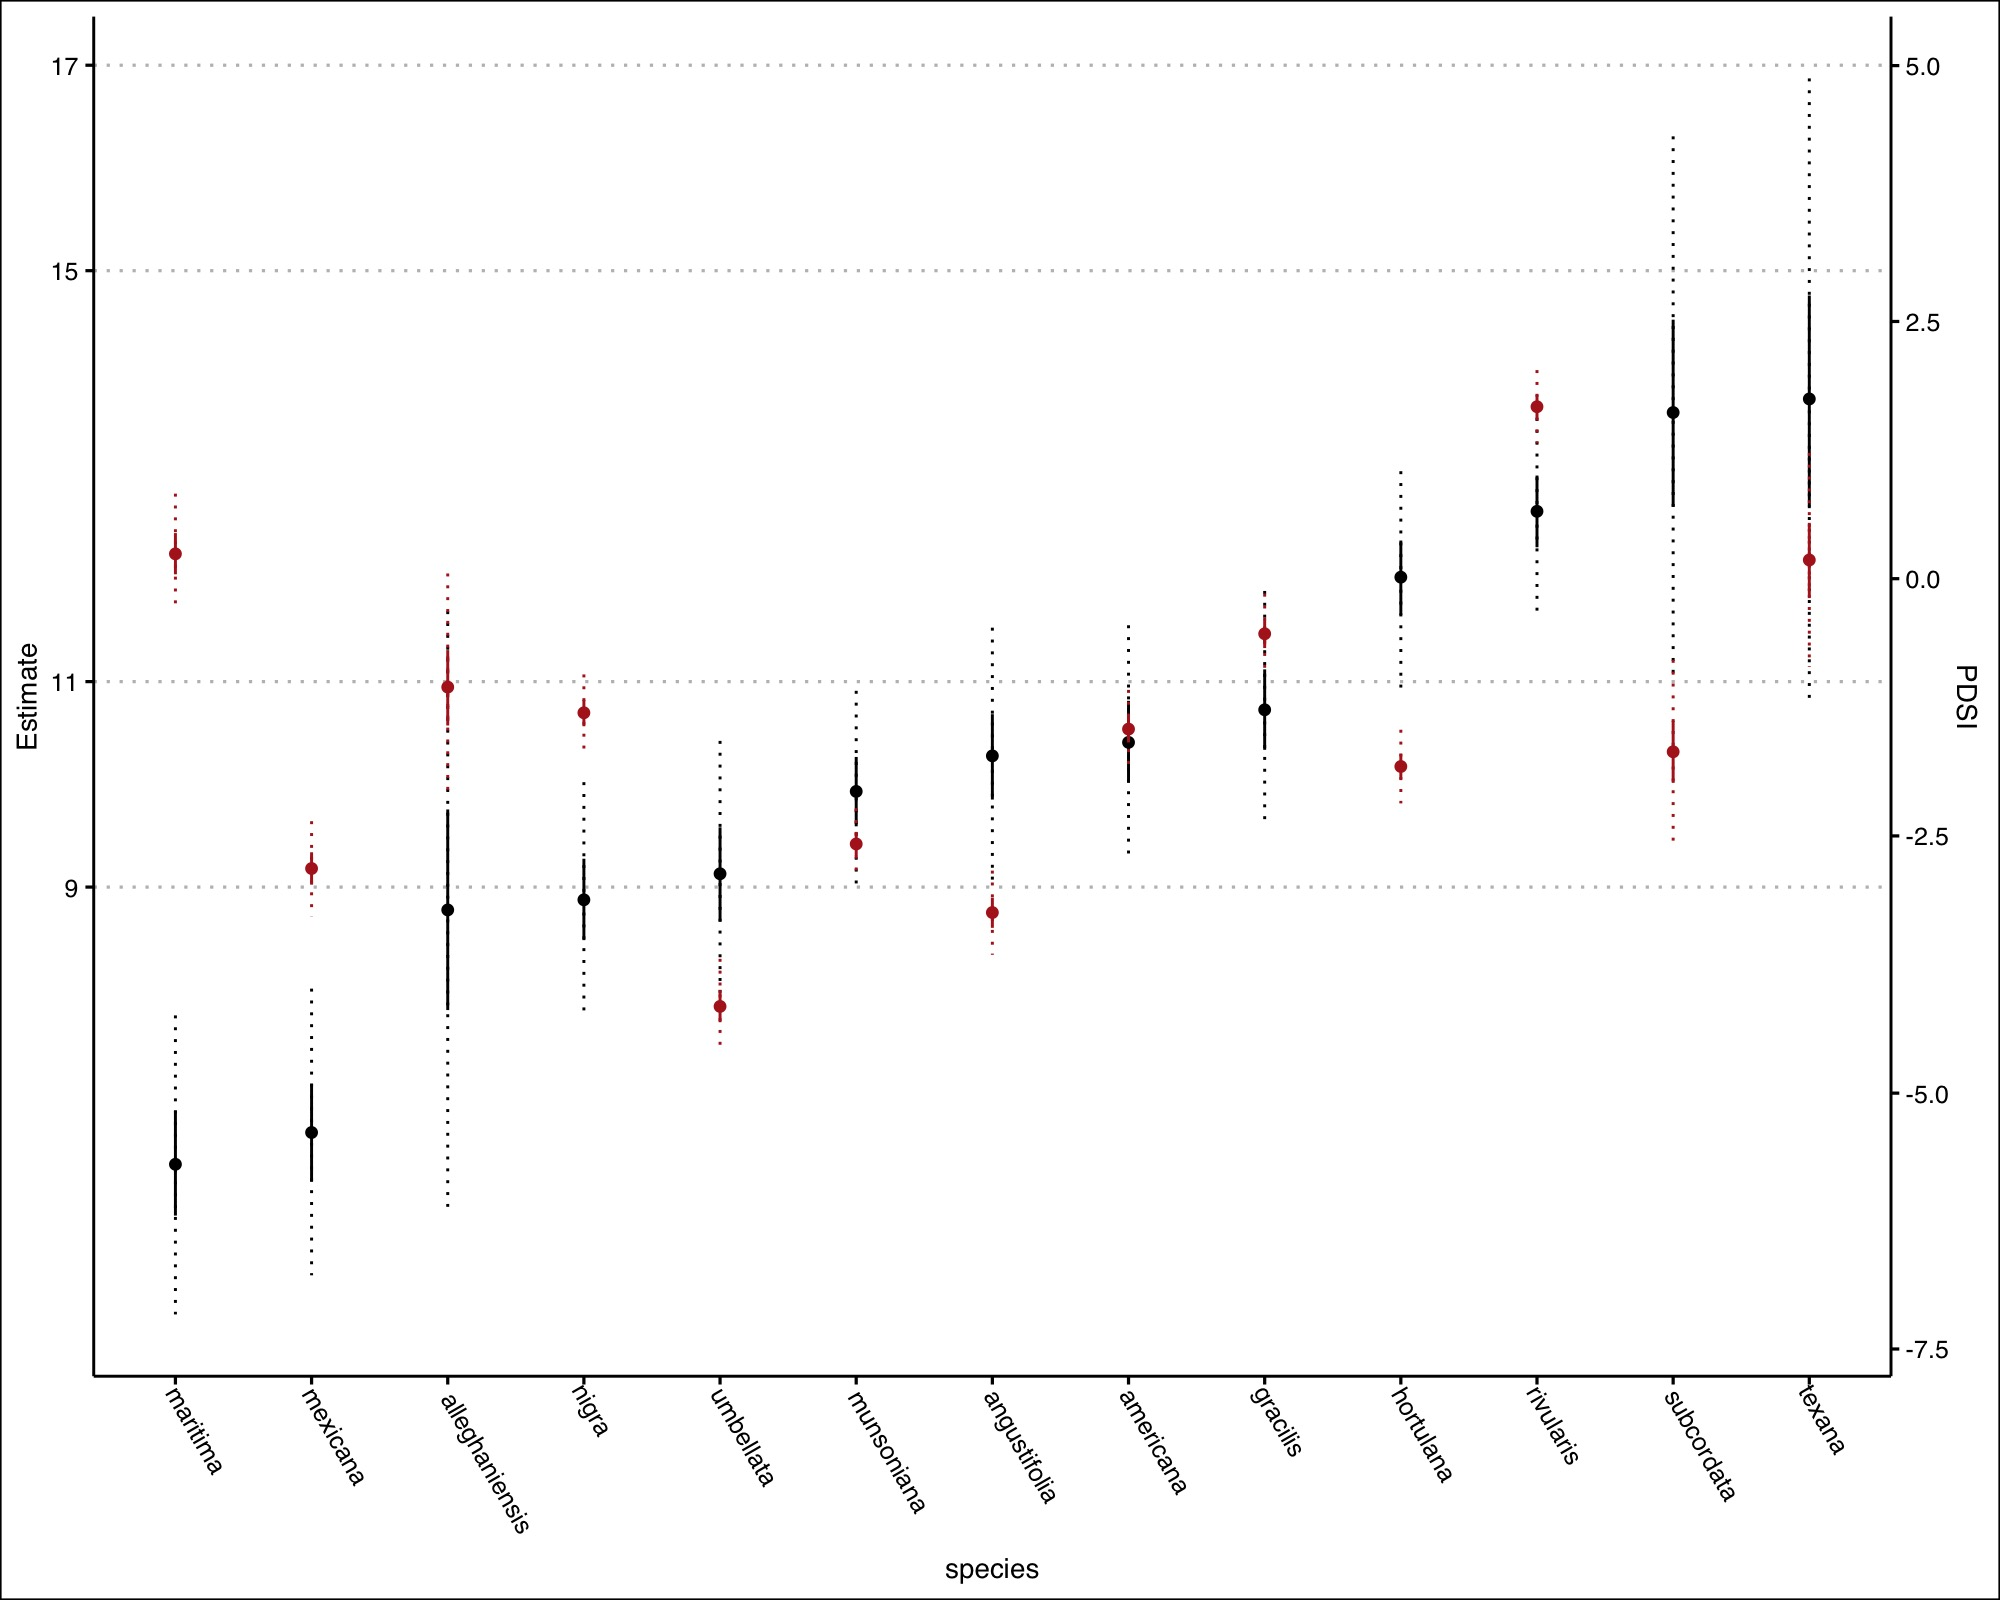
\includegraphics[width=\textwidth]{..//Plots/pdsi.jpeg}
                 \caption{Modeled PDSI (red) and FLS (black) for each species plotted on same axis. Next step: Joint model}
    \end{figure}

\subsection*{FLS and Climate Change}    
    
   \begin{figure}[h!]
        \centering
         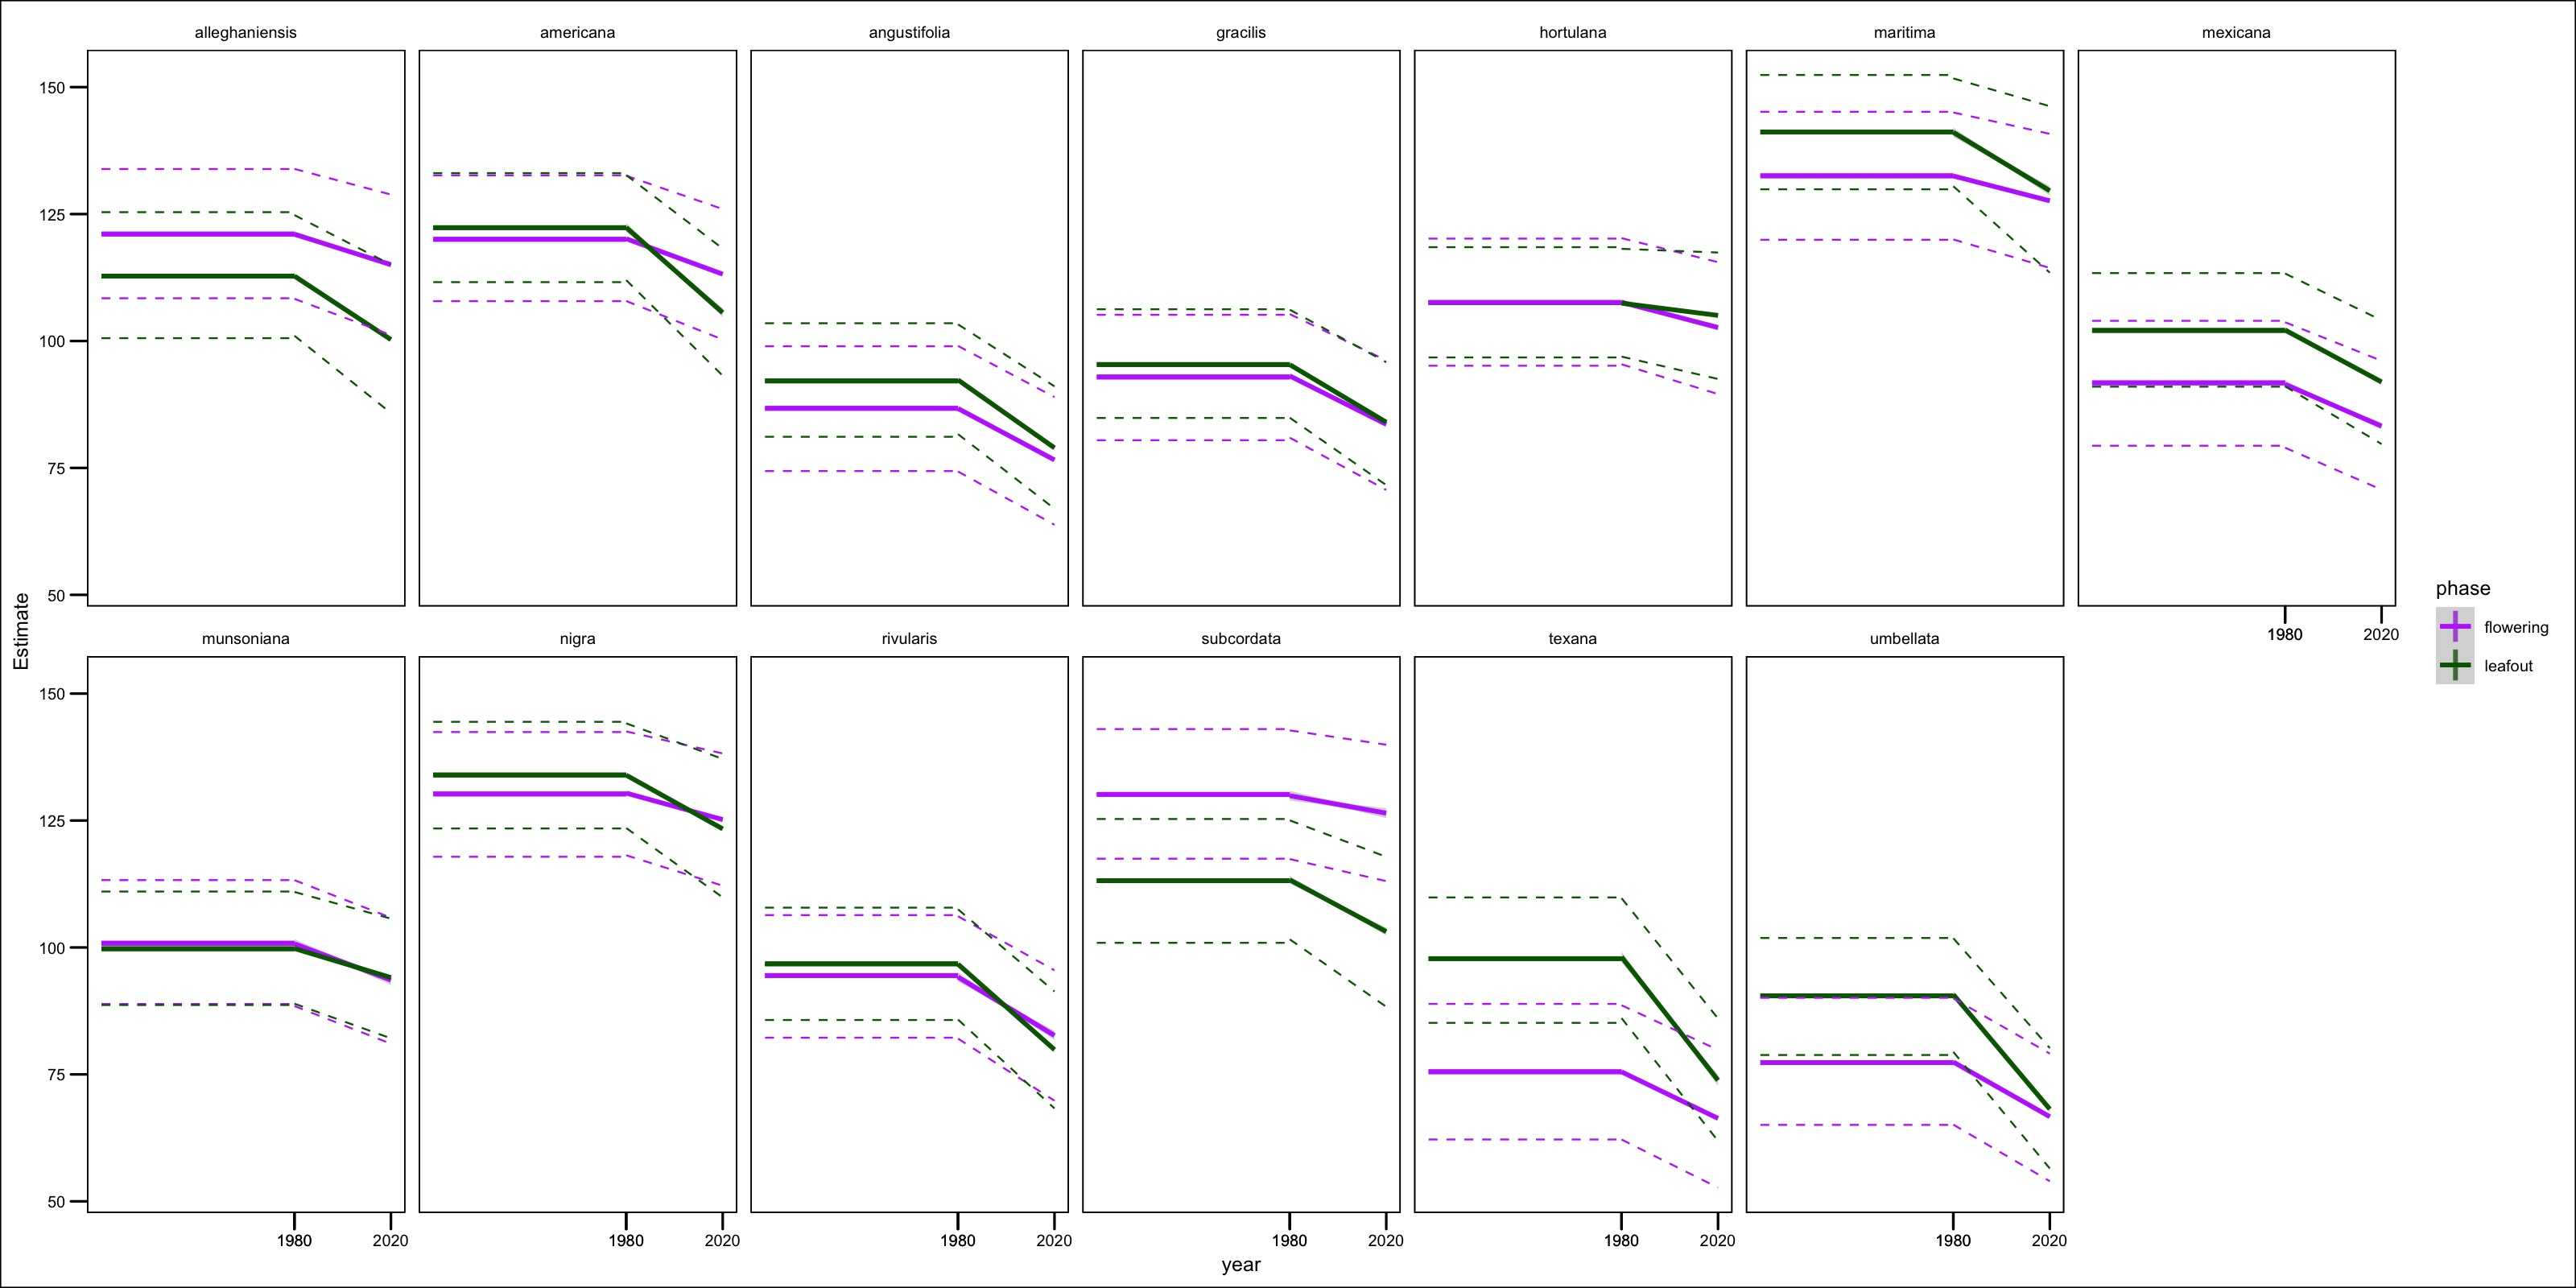
\includegraphics[width=\textwidth]{..//Plots/climchange.jpeg}
                 \caption{Seems like leaves are more sensitive than flowers}
    \end{figure}


\end{document}
